\documentclass[12pt, french, latin.medieval, a4paper]{report}
% package de langues 
\usepackage[french]{babel}
\usepackage[utf8]{inputenc}
\usepackage[T1]{fontenc}

% package pour référence de liens sur pdf 
\usepackage[pdftex]{hyperref} % liens
\usepackage{lastpage} % numéro de page
\usepackage{caption}

% package de formes de document 
\usepackage[left=2.5cm,
              right=2.5cm,
              top=2.5cm,
              bottom=2.5cm
             ]{geometry}
% pour les tableaux 
\usepackage{array,multirow,makecell} 
\newcolumntype{R}[1]{>{\raggedleft\arraybackslash }b{#1}}
\newcolumntype{L}[1]{>{\raggedright\arraybackslash }b{#1}}
\newcolumntype{C}[1]{>{\centering\arraybackslash }b{#1}}

% package pour la page de couverture 
\usepackage{graphicx}
\usepackage[cyr]{aeguill}
\usepackage{fancyheadings}
\usepackage{amsmath}
\usepackage{amsfonts}
\usepackage{amssymb}
\usepackage{geometry}
\usepackage{eso-pic}
\usepackage{tikz}
\usetikzlibrary{calc}


% nouvelle commande pour la forme 
%\fancyhf[OFC]{\thepage / \pageref{LastPage}}
\rfoot{\thepage / \pageref{LastPage}}
%\setcounter{tocdepth}{3}

% pakages de couleurs du document
\usepackage{color}
\usepackage{xcolor}


% package pour la chimie
\usepackage[version=4]{mhchem}


% package pour la visualisation du code
\usepackage{listings}
\definecolor{darkWhite}{rgb}{0.94,0.94,0.94}
 
\lstset{
  aboveskip=3mm,
  belowskip=-2mm,
  backgroundcolor=\color{darkWhite},
  basicstyle=\footnotesize,
  breakatwhitespace=false,
  breaklines=true,
  captionpos=b,
  commentstyle=\color{red},
  deletekeywords={...},
  escapeinside={\%*}{*)},
  extendedchars=true,
  framexleftmargin=16pt,
  framextopmargin=3pt,
  framexbottommargin=6pt,
  frame=tb,
  keepspaces=true,
  keywordstyle=\color{blue},
  language=python,
  literate=
  {²}{{\textsuperscript{2}}}1
  {⁴}{{\textsuperscript{4}}}1
  {⁶}{{\textsuperscript{6}}}1
  {⁸}{{\textsuperscript{8}}}1
  {€}{{\euro{}}}1
  {é}{{\'e}}1
  {è}{{\`{e}}}1
  {ê}{{\^{e}}}1
  {ë}{{\¨{e}}}1
  {É}{{\'{E}}}1
  {Ê}{{\^{E}}}1
  {û}{{\^{u}}}1
  {ù}{{\`{u}}}1
  {â}{{\^{a}}}1
  {à}{{\`{a}}}1
  {á}{{\'{a}}}1
  {ã}{{\~{a}}}1
  {Á}{{\'{A}}}1
  {Â}{{\^{A}}}1
  {Ã}{{\~{A}}}1
  {ç}{{\c{c}}}1
  {Ç}{{\c{C}}}1
  {õ}{{\~{o}}}1
  {ó}{{\'{o}}}1
  {ô}{{\^{o}}}1
  {Õ}{{\~{O}}}1
  {Ó}{{\'{O}}}1
  {Ô}{{\^{O}}}1
  {î}{{\^{i}}}1
  {Î}{{\^{I}}}1
  {í}{{\'{i}}}1
  {Í}{{\~{Í}}}1,
  morekeywords={*,...},
  numbers=left,
  numbersep=10pt,
  numberstyle=\tiny\color{black},
  rulecolor=\color{black},
  showspaces=false,
  showstringspaces=false,
  showtabs=false,
  stepnumber=1,
  stringstyle=\color{gray},
  tabsize=4,
  title=\lstname,
}

%package pour les algorithmes
\usepackage{algorithm}
\usepackage{algorithmic}
\usepackage{amsmath}

% package pour les tableaux
\usepackage{longtable}
\usepackage{booktabs}

% package pour les figures 
\usepackage{subcaption}

% package de reférencement
% \usepackage[backend=biber,safeinputenc, sorting=none]{biblatex}

% mettre la bibliographie dans la table de matières
%\usepackage[nottoc, notlof, notlot]{tocbibind}
\include{page_couverture.tex}


\author{MBE MBE MINDJANA LOIC HENRI}
\title{GNPS et MDByTE}

\begin{document}
    
    \pagecouverture
    {Clustering : clustering par modélisation et par densité}
    {}
    \tableofcontents
    \vspace{20cm}
    
    \section{Introduction}
        Ces dernières années, les algorithmes de clustering connaissent une certaine popularité du fait de leur utilisation dans plusieurs domaines d’activités tel que le domaine des finances, de la vision par ordinateur, de l’éducation, du marketing etc... Ils sont communément utilisés dans l’exploration de grandes quantités de données dans le but d’extraire et ressortir des structures, des informations qui y sont contenues et qui seraient difficile à obtenir uniquement en réalisant une analyse directe. Qu’est-ce que le clustering ? Et quels sont les différents types d’algorithmes de clustering ? Peut-on utiliser ces algorithmes pour des données spectrales ? Dans le but de répondre à ces questions, nous parlerons du clustering dans sa globalité et par la suite du clustering par modélisation et par densité qui en sont des types spécifiques.

    \section{Clustering}
    Le clustering est un processus d'analyse exploratoire qui consiste sur la base d’un ensemble de données (communément appelées observations ou points), à regrouper ceux qui sont similaires entre eux. Cette opération de regroupement amène à obtenir des groupes d’observations appelés clusters dans lesquels se trouvent des observations qui sont similaires les uns, des autres.
    
    Plus formellement, soit $X = { x_1, x_2, ..., x_n }$ un ensemble de $n$ observations que nous souhaitons regrouper en un nombre $K$ de clusters connus ou non. Faire du clustering revient à trouver une fonction $f: X \to \{1..i..K\}$ où $i$ est l'indicateur du cluster $C_i$. tel que $\forall x_1,\  x_2\ \in C_i$ et $\forall x_3 \in C_j$, on a:

    \begin{itemize}
        \item $sim(x_1, x_2) > sim(x_1, x_3)$
        \item $sim(x_1, x_2) > sim(x_2, x_3)$
    \end{itemize}
    $sim$ étant une mésure de similarité entre deux observations.    

    \begin{figure}
        \centering
        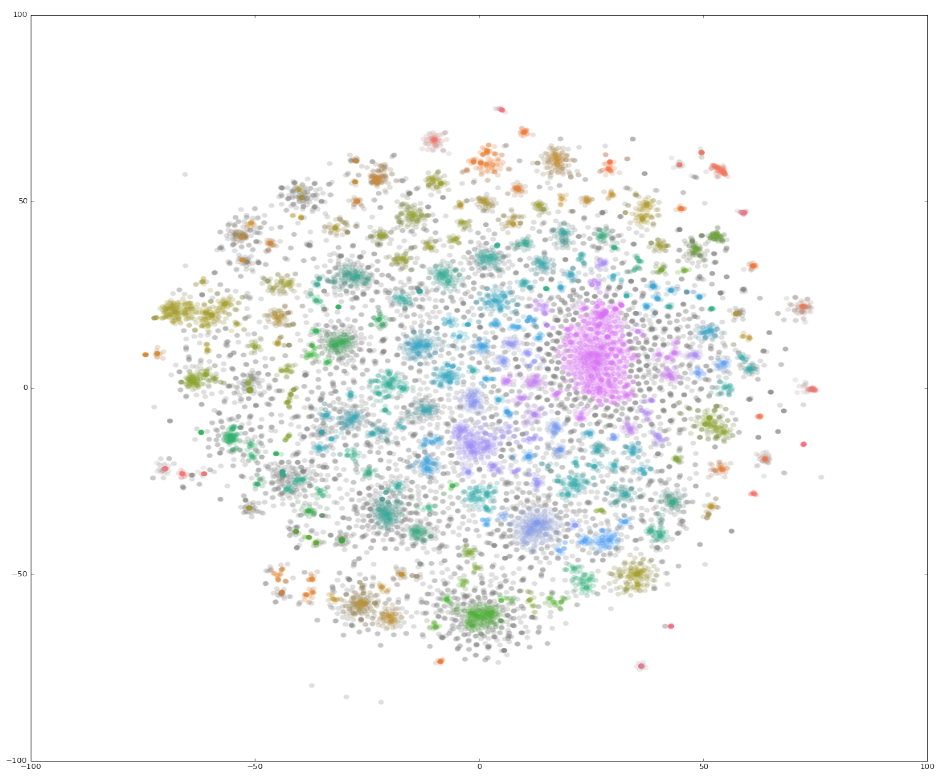
\includegraphics[width= \linewidth]{Images/490cf86a.png}
        \caption{Clustering des données de MNIST \href{https://www.ons.gov.uk/methodology/methodologicalpublications/generalmethodology/onsworkingpaperseries/onsworkingpaperseriesnumber14unsuperviseddocumentclusteringwithclustertopicidentification}{1}}
        \label{fig:clustering}
    \end{figure}
    Les notions de similarité et de dissimilarité sont donc importantes à définir. Afin de mesurer une similarité, on doit définir une mesure $s$ qui devra répondre aux exigences suivantes:

    \begin{enumerate}
        \item $\forall x, y \in X, sim(x,y) = sim(y,x)$.
        \item $\forall x, y \in X, sim(x,y) \geq 0$.
        \item $\forall x \in X, sim(x,x) = 1$.
        \item $\forall x, y \in X, sim(x,y) = 1 \Leftrightarrow x = y$.
    \end{enumerate}

    Comme mesures de similarité les plus utilisées et les plus connues, on a: 
    \begin{itemize}
        \item \textbf{Cosinus de similarité} : $sim(x,y) = \frac{x \cdot y}{\|x\| \|y\|}$
        \item \textbf{Indice de Jaccard} : $sim(x,y) = \frac{|x \cap y|}{|x \cup y|}$
    \end{itemize}
    
    Pour mesurer la dissimilarité, on doit définir une mesure de distance $d$ qui devra répondre plutôt aux exigences suivantes:

    \begin{enumerate}
        \item $\forall x, y \in X, d(x,y) = d(y,x)$.
        \item $\forall x, y \in X, d(x,y) \geq 0$.
        \item $\forall x \in X, d(x,x) = 0$.
        \item $\forall x, y \in X, d(x,y) = 0 \Leftrightarrow x = y$.
    \end{enumerate}

    Comme mesures de distances communément utilisées, on peut citer :
    \begin{itemize}
        \item \textbf{Distance euclidienne} : $d(x,y) = \sqrt{\sum_{i=1}^{n}(x_i - y_i)^2}$
        \item \textbf{Distance de Manathan} : $d(x,y) = \sum_{i=1}^{n}|x_i - y_i|$
        \item \textbf{Distance de Minkwoski} : $d(x,y) = \left(\sum_{i=1}^{n}|x_i - y_i|^p\right)^{\frac{1}{p}}$
    \end{itemize}
    
    Plusieurs approches de construction de clusters ou de regroupement d’observations ont vue le jour, ce qui a conduit à la création de divers algorithmes de clustering, qui peuvent ètre regrouper en les types de clustering suivant :

    \begin{itemize}
        \item \textbf{Clustering par partitionement}: On cherche à construire des clusters qui seront disjoints entre eux et dont séparés, ce qui conduit à partitionner ou encore à diviser l’ensemble des observations, le plus commun de ce type d’algorithmes est l’algorithme KMEANS.  En pratique de tels algorithmes sont très utiles lorsque les données forment naturellement des groupes à forme sphérique, ne contiennent pas ou presque pas de bruits et ne possèdent pas d’outliers (qui sont des observations non communs). Il faut noter que les bruits peuvent survenir du matériel de création de la donnée, du processus de création de la donnée et même des approximations faites.
        
        \item \textbf{Clustering hiérarchique} : L’approche est de construire une hiérarchie de clusters des données, de façon ascendante ou descendante. Ascendante selon le fait qu’on débute la construction depuis chaque observation, et descendante en revanche en partant de tout l’ensemble des observations. Comme algorithmes les plus utilisés, on a l’algorithme de classification ascendante hiérarchique (CAH) et la classification descendante hiérarchique (CDH). Des algorithmes pareils sont très utilisés pour construire et définir des hiérarchies entre les données sans toutefois connaitre le nombre de clusters à l’avance, mais sont également sensibles aux bruits et aux outliers.

        \item \textbf{Clustering par modélisation} : l’idée est de construire des clusters qui seront modélisés d’une certaine manière. Communément les clusters sont modélisés par des modèles probabilistes, ce qui est le cas pour l’algorithme de modèle de mélanges gaussien (GMM). En pratique ces types d’algorithmes sont plus résistants aux données contenant des bruits et des outliers. L’avantage principale de ces algorithmes est qu’ils permettent de découvrir des structures sous-jacentes des données obtenues des modèles probabilistes.

        \item \textbf{Clustering par densité} : L’approche est celui d’identifier une zone d’observations à forte densité comme étant un cluster d’observations. Les algorithmes DBSCAN(Density-Based Spatial Clustering of Applications With Noise) et OPTICS y sont les algorithmes les plus utilisés. Comme ceux du clustering par modélisation, ces algorithmes sont résistants aux bruits.
        
    \end{itemize}

    Les données spectrales tel que les spectres MS/MS et RMN pouvant être impactées respectivement par la qualité de l’ionisation utilisés et les matériaux utilisés pour leurs constructions, peuvent fortement avoir des bruits. De ce fait utiliser des algorithmes de clustering par modélisation ou par densité sur de tel données semble être logique. Nous parlerons ainsi dans la suite, plus spécifiquement du clustering par modélisation et par densité.

    \section{Clustering par modélisation}
        Comme décrit dans la section précédente, le clustering par modélisation consiste à regrouper des observations tout en modélisant les clusters. Plusieurs algorithmes de clustering par modélisation ont été créés à l'instar de:
        
        \begin{itemize}
            \item l'algorithme \textbf{GMM} (Gaussian Mixture Model) : on modélise les clusters par des observations suivant des distributions gaussiennes
            \item l'algorithme \textbf{LDA} (Latent Dirichlet Allocation) : on modélise des clusters comme un ensemble de sujets latents.
        \end{itemize}
        
        \subsection{Algorithme GMM}
            L'algorithme de GMM (Gaussian Mixture Model) \cite{dempster1977maximum} est un algorithme de clustering qui permet de modéliser des données par un mélange de distributions gaussiennes \ref{fig:gmm}. Il cherche sur la base des différents paramètres des distributions gaussienes à maximiser la vraissemblance $\Lambda(X)$ des données $X$ qui est en fait la probabilité que des données soient générées par un modèle et ses paramètres. 
            Soient $x$ une observation, et $p(x)$ la fonction qualifiée de loi marginale, permettant d'évaluer la probabilité d'obtenir $x$ depuis $X$ l'ensemble des observations possibles et le modèle.
            Nous savons que :
            \begin{equation}
                p(x) = \sum_{k=1}^{K} p(x,C=C_k) = \sum_{k=1}^{K} p(C=C_k)p(x|C=C_k)
            \end{equation}

            Sachant qu'un cluster est un ensemble d'observations suivant une distribution gaussienne, on aura en notant $\pi_k = p(C=C_k)$ :
            \begin{equation}
                p(x) = \sum_{k=1}^{K} \pi_k \times N(x, \mu_{k}, \sigma_{k})
            \end{equation}
            \begin{equation}
                N(x, \mu, \sigma) = \frac{1}{|\sigma| \sqrt{(2\pi)^d}} e^{-\frac{1}{2}(x-\mu){\sigma}^{-1}(x-\mu)} \text{où $d$ est la taille d'une donnée $x$}
            \end{equation}
        
            La vraissemblance $\Lambda(X)$ de la distribution des données $X$ est égale à:
            \begin{equation}
            \Lambda(X) = \prod_{x \in X} p(x)
            \end{equation}
            \begin{equation}
                \log(\Lambda(X)) = \sum_{x \in X} log(p(x)) =  \sum_{x \in X} log(\sum_{k=1}^{K} \pi_k \times N(x, \mu_{k}, \sigma_{k}))
            \end{equation}
            
            En sachant que chacune des observations sera associée à un cluster. on aura le logarithme de la vraissemblance complété étant:
            \begin{equation}
                \log_c(\Lambda(X)) = \sum_{x \in X}\sum_{k=1}^{K} p(C=C_{k}|x) \times log(\pi_k \times N(x, \mu_{k}, \sigma_{k}))
            \end{equation}
            En notant $\gamma_{k}(x) = p(C=C_{k}|x)$, on a :
            \begin{equation}
                \log_c(\Lambda(X)) = \sum_{x \in X}\sum_{k=1}^{K} \gamma_{k}(x) \times log(\pi_k \times N(x, \mu_{k}, \sigma_{k}))
            \end{equation}

            On souhaite donc obtenir $\theta = (\pi, \mu, \sigma)$ qui maximise $\log_c(\Lambda(X))$ ou tout simplement minimise $-\log_c(\Lambda(X))$. Vue qu'on n'a pas de conditions sur $\theta$ et que $-\log_c(\Lambda(X))$ est convexe alors la solution est obtenu lorsque le gradient de $-\log_c(\Lambda(X))$ est nulle, c'est à dire:
            \begin{equation}
                \nabla\log_c(\Lambda(X)) = 0
            \end{equation}
            De là on tire les formules de valeurs optimales $\hat{\theta}$ suivantes:

            \begin{equation}
                \hat{\mu_{k}}= \frac{\sum_{x \in X} \gamma_{k}(x) x}{\sum_{x \in X} \gamma_{k}(x)}
                \label{equa:gmm1}
            \end{equation}
            \begin{equation}
                \hat{\pi_{k}}= \frac{\sum_{x \in X} \gamma_{k}(x)}{|X|}
                 \label{equa:gmm2}
            \end{equation}

            \begin{equation}
                \hat{\sigma_{k}}= \frac{\sum_{x \in X} \gamma_{k}(x -\hat{\mu_{k}}){(x -\hat{\mu_{k}})}^T}{\sum_{x \in X} \gamma_{k}(x)}
                 \label{equa:gmm3}
            \end{equation}

            De ces formules, on peut remarquer que pour maximiser la log-vraissemblance complétée, il faut préalablement calculer $\gamma_{k}(x)$. Afin de s'assurer que ces calculs ne posent pas problème pour optimiser globalement la log-vraissemblance complétée, l'algorithme EM(Expectation - Maximisation) \ref{alg:gmm} est utilisé.
            
            \begin{figure}
                \centering
                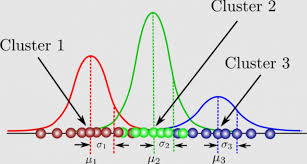
\includegraphics{Images/gmm.jpeg}
                \caption{Modélisation de clusters par des gaussienes \href{https://vitalflux.com/gaussian-mixture-models-what-are-they-when-to-use}{1}}
                \label{fig:gmm}
            \end{figure}
            
            \begin{algorithm}[H]
             \caption{Pseudo code de GMM}
             \label{alg:gmm}
             \begin{algorithmic}[1]
              \REQUIRE Données d'entrée $X$, nombre de clusters $K$
              \ENSURE Clusters $C$
              \STATE Initialiser les paramètres du modèle $\theta = (\pi, \mu, \sigma)$
              \WHILE{non convergence}
                \STATE Calculer les probabilités $\gamma_{k}(x)$ pour toutes les observations $x$
                \STATE Mettre à jour les paramètres $\theta = (\pi, \mu, \sigma)$ du modèle en maximisant la log-vraisemblance complétée $\log_c(\Lambda(X))$ par les équations \ref{equa:gmm1}, \ref{equa:gmm2} et \ref{equa:gmm3}
              \ENDWHILE
              \STATE Assigner chaque observation $x$ au cluster $C_k$ avec la plus grande probabilité $\gamma_{k}(x)$
             \end{algorithmic}
            \end{algorithm}

            Cet algorithme GMM par le biais de la pseudo reconstruction de la distribution des données permet d'identifier si une observation est potentiellement un bruit ou encore un outlier. Il permet d'avoir une vue probabiliste des observations suivant la loi gaussienne, qui permet d'avoir une connaissance du domaine dans lequel les observations ont été obtenus.
        
            
    \section{Clustering par densité}
        Comme décrit dans la rubrique de clustering, le clustering par densité consiste à définir un cluster comme une zone à forte densité d'observations. Cette densité est généralement mesurée par:
        
        \begin{itemize}
            \item un paramètre de voisinage $\epsilon$ qui permet pour une observation $x$ d'obtenir une liste de ses voisins $x'$ telque $d(x, x') <= \epsilon$ (on pourrait utiliser une mésure de similarité). Cette liste constitue le voisinage d'une observation
            \item un paramètre de limitation $MinPts$ qui permet de définir une borne à partir de laquelle on considère que le voisinage d'une observation est dense.
        \end{itemize}  
        On peut citer de ce type d'algorithmes de clustering :
        \begin{itemize}
            \item l'algorithme \textbf{DBSCAN} (Density-Based Spatial Clustering of Applications with Noise) : utilise les paramètres $\epsilon$ et $MinPts$ pour regrouper des observations en des zones de densité
            \item l'algorithme \textbf{HDBSCAN} (Hierachical Density-Based Spatial Clustering of Applications with Noise) est une amélioration de DBSCAN introduisant l'hierachisation de clusters 
        \end{itemize}

        \subsection{Algorithme de DBSCAN}
            DBSCAN (Density-Based Spatial Clustering of Applications with Noise) \cite{khan2014dbscan} est un algorithme de clustering utilisé pour regrouper des points de données similaires en définissant un cluster comme une zone à grande densité. Définir un cluster comme une zone à forte densité permet implicitement de ne pas définir le nombre $K$ de clusters à l'avance, vue qu'il peut ètre trouvé en meme temps que les clusters.
    
            Soit $N(x, \epsilon)$ l'ensemble des observations voisins de l'observation $x$ étant dans le rayon $\epsilon$, on a :
    
            \begin{equation}
                N(x, \epsilon) = \{ x' | d(x', x) \leq \epsilon\}
            \end{equation}
    
            L'algorithme DBSCAN s'appuie sur des types d'observations \ref{fig:mod_dbscan} pour pouvoir construire les clusters:
            \begin{itemize}
                \item \textbf{Core Point} : est une observation coeur caractérisée par le fait que le nombre de ses voisins dépasse le seuil de points minimun $MinPts$. Il permet de détecter une zone dense
                \item \textbf{Border Point} : est une observation appartenant au voisinage d'un \textbf{Core Point} mais ne l'est pas. Il permet de définir la limite d'une zone dense
                \item \textbf{Noise Point} : est une observation qui n'est ni \textbf{Core Point}, ni \textbf{Border Point}. Il est une observation séparée des autres, qu'on peut qualifiée de bruits et meme d'outliers.
            \end{itemize}
            
            \begin{figure}
                \centering
                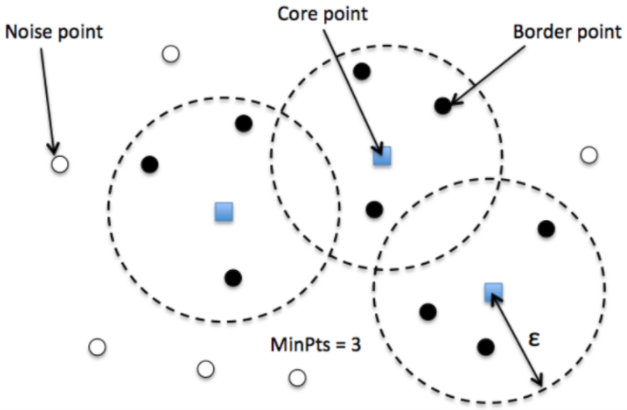
\includegraphics[width=\linewidth]{Images/dbscan.png}
                \caption{Types clés d'observations de DBSCAN}
                \label{fig:mod_dbscan}
            \end{figure}
    
            \begin{algorithm}[H]
                \caption{Pseudo code de DBSCAN}
                \label{alg:dbscan}
                \begin{algorithmic}[1]
                \REQUIRE Ensemble de données $X$, rayon de voisinage $\epsilon$, nombre minimum de points $MinPts$
               \ENSURE Clusters $C$
                
                \FORALL{point $x$ de $X$}
                    \IF{$ N(x, \epsilon) \geq MinPts$}
                        \STATE Marquez $x$ comme  \textit{visité}
                        \STATE Creez un cluster $c$ et ajoutez $x$ à $c$
                        \STATE Ajouter tous les points de $N(x, \epsilon)$ qui n'ont pas encore été \textit{visités} à $c$ et affecter les à $STACK$
                        \WHILE{$STACK$ n'est pas vide}
                            \STATE $x' \leftarrow pop(STACK)$
                            \IF{ $ N(x', \epsilon) \geq MinPts$}
                                \STATE Marquez $x'$ comme \textit{visité}
                                \STATE Ajouter tous les points $N(x', \epsilon)$ qui n'ont pas encore été \textit{visités} à $c$ et à $STACK$ et marquer ces points comme \textit{visités}. 
                                \ENDIF
                            \ENDWHILE
                        \ELSE
                            \STATE Marquer $x$ comme \textit{Noise Point} et \textit{visité}.
                        \ENDIF
                \ENDFOR
                \end{algorithmic}
            \end{algorithm}
    
            De part le pseudo code, on peut comprendre intuitivement pourquoi l'algorithme permet de détecter des bruits ou encore les outliers. Cette capacité de l'algorithme à pouvoir détecter ces points est une force qui malheuresement dépend fortement de la distance choisie, du paramètre $\epsilon$ et surtout du minimun de points $MinPts$ permettant de détecter une zone dense. Toutefois il ne faut oublié qu'il permet d'éviter de construire des clusters sans pour autant définir le nombre de clusters à l'avance. De plus l'algorithme peut ètre modifé, au niveau de la définition des voisinages d'observations en utilisant une mesure de similarité au lieu d'une distance et en voyant $\epsilon$ comme seuil de similarité, ce qui rapprochera le clustering, d'une construction de réseau moléculaire (dans le cas où on a des données spectrales MS/MS par exemple).
                
        
\section{Conclusion}

    En définitive, nous avons parlé du clustering dans son ensemble, des types de clustering, plus précisément du clustering par modélisation et par densité. Il était question pour nous dans ce document de parler plus spécifiquement des algorithmes de clustering par modélisation et par densité et de mettre en évidence la raison de faire le choisir de tel algorithmes pour regrouper et apprendre des structures des données spectrales MS ou RMN compte tenu de leurs natures. On peut noter que ces algorithmes de clustering, comme d’autres présentés n’utilisent des données que de même environnement. C’est-à-dire si les données sont constituées de spectres MS et RMN pour chaque observation alors les regroupements ne se feront pas conjointement selon ces types de spectres. Ils seront faits soit en concaténant les spectres, soit en les utilisant différemment; ce qui ne nous permet pas d’exploiter le fait d’avoir ces vues (spectre MS et spectre RMN) pour de tel données. D’où l’interrogation existe-t-il des algorithmes de clustering qui s’appuient sur des données ayant plusieurs vues ?

\bibliographystyle{plain}
    \bibliography{reference_GNPS_MADByTE}
\end{document}